\section{Processi di Supporto}

	\subsection{Documentazione}
		\subsubsection{Descrizione}
			In questo capitolo sono presenti le norme adottate per 	redigere, verificare e approvare la documentazione ufficiale prodotta da Dream Corp. Tutti documenti sono elencati nella sezione \hyperref[3.1.5]{\textit{\underline{3.1.5}}} denominata "Lista documenti".
		\subsubsection{Divisione dei documenti}
			Per una maggiore formalità ogni documento è stato classificato in Interno o Esterno in base alle seguenti caratteristiche:
			\begin{itemize}
				\item \textbf{Interno:} ha utilità interna al team, ovvero contiene tutte le informazioni significative per componenti del gruppo in fase di sviluppo;
				\item \textbf{Esterno:} condiviso anche con i Committenti e la Proponente, espone le informazioni utili per spiegare il metodo di lavoro seguito per lo sviluppo del progetto.
			\end{itemize}
		\subsubsection{Nomenclatura}
			I documenti formali seguono uno standard preciso per la loro nomenclatura. Di seguito un esempio esplicativo: 					\newline 
			\begin{center}
				DocumentoDiEsempio.for
			\end{center}
			\begin{itemize}
				\item \textbf{DocumentoDiEsempio:} indica il nome del documento che viene scritto utilizzando la lettera maiuscola per ogni parola presente senza spazi al suo interno;
				\item \textbf{.for:} indica il formato del documento. Quest'ultimo sarà \textit{.tex} dalla fase di creazione fino alla sua approvazione e da quel momento in poi verrà creato il file \textit{.pdf} contenente la versione definitiva di quel documento.
			\end{itemize}
			\textbf{Codice per il versionamento} La versione del documento è specificata all'interno del documento stesso in una tabella dove sono segnate in modo preciso tutte le modifiche fatte fino ad arrivare alla major release in formato PDF. Il sistema utilizzato verrà spiegato in modo più dettagliato successivamente nella sezione \hyperref[3.2.2]{\textit{\underline{3.2.2}}} di questo documento.
		\subsubsection{Ciclo di vita documentazione}
			Per ogni documento formale sono previste tre fasi obbligatorie:
			\begin{itemize}
			\item \textbf{Redazione:} questa fase dura dalla creazione del documento fino alla scrittura completa di tutti i contenuti previsti. Durante questo processo, il Responsabile di Progetto assegna ai Redattori i contenuti da aggiungere e una volta che quest'ultimi saranno esauriti potrà approvare il passaggio alla fase successiva;
			\item \textbf{Verifica:} in questa fase il documento viene controllato in ogni sua parte attraverso le opportune procedure dai Verificatori che una volta ultimato il lavoro daranno il loro feedback al Responsabile di Progetto; questo può dunque approvare il documento che passa quindi alla fase successiva oppure può farlo tornare alla fase di Redazione per correggere eventuali imperfezioni riscontrate dai Verificatori;
			\item \textbf{Approvato:} In questa fase il documento è pronto per essere rilasciato e la sua versione viene aggiornata ad una major.
			\end{itemize}
		\subsubsection{Lista documenti}
		\label{3.1.5}
			\begin{itemize}
				\item \textbf{Analisi dei Requisiti: }[Esterno] \newline
				Il suo scopo è di analizzare ed esporre i requisiti del progetto. Contiene l'analisi dei casi d'uso che riguardano il prodotto in fase di sviluppo e i diagrammi di interazione con l'utente a prodotto ultimato;
				\item \textbf{Norme di Progetto: }[Interno] \newline
				Contiene tutte le regole e le convenzioni adottate dai membri del gruppo Dream Corp. per uno sviluppo metodico del progetto;
				\item \textbf{Piano di Progetto: }[Esterno] \newline
				Il suo scopo è quello di descrivere gli obiettivi del progetto e gli elementi necessari per il loro raggiungimento. Inoltre, vien presentato come il gruppo Dream Corp. amministra il proprio tempo e i membri al suo interno;
				\item \textbf{Piano di Qualifica: }[Esterno] \newline
				Consiste in una spiegazione dettagliata di come il team Dream Corp. vuole soddisfare i requisiti di qualità del progetto;
				\item \textbf{Studio di Fattibilità: }[Interno] \newline
				Il suo obiettivo è di mostrare come è stato analizzato ogni capitolato elencando per ognuno punti a favore e sfavore in modo da evidenziare tutti i dubbi sorti in fase di decisione.
				\item \textbf{Glossario: }[Esterno] \newline
				Contiene tutti i termini presenti nei documenti formali che il gruppo Dream Corp. ha ritenuto opportuno avessero bisogno di una spiegazione o chiarimento per facilitarne la comprensione. è unico per tutti i documenti.
			\end{itemize}
		\subsubsection{Norme tipografiche}
			Le norme scritte in questa sezione devono essere seguite in tutti i documenti prodotti dal team Dream Corp.:
			\begin{itemize}
				\item \textbf{Date:} sono scritte seguendo la regola anno-mese-giorno (DD-MM-YYYY);
				\item \textbf{Voci nel Glossario:} per segnalare una parola che si trova nel glossario viene posta una \textbf{G} a pedice della parola;
				\item \textbf{Link interni:} i collegamenti che rimandano a una sezione interna al documento sono scritti in corsivo e sottolineati;
				\item \textbf{Link esterni:} i collegamenti che rimandano a una pagina web esterna al documento sono scritti in colore blu;
				\item \textbf{Elenchi puntati:} ogni elemento della lista è caratterizzato in generale da una prima parola o serie di parole in grassetto seguite da due punti \textit{":"} e successivamente dal suo contenuto, ma può anche essere formato solamente dal contenuto nei casi in cui non sia necessaria una particolare specifica iniziale. Alla fine è posto un punto e virgola \textit{";"} tranne per l'ultimo elemento che è concluso da un punto \textit{"."};
				\item \textbf{Citazioni:} le citazioni sono scritte in \textit{corsivo}.
			\end{itemize}
		\subsubsection{Struttura dei documenti}
			Tutti i documenti utilizzano una struttura di base contenuta nel file \textit{stile.tex} in modo da non ripetere ogni volta gli elementi comuni.
			\newline \newline \textbf{Frontespizio} È la prima pagina del documento dove si trovano:
			\begin{itemize}
				\item \textbf{Logo:} immagine identificativa del gruppo;
				\item \textbf{Nome del progetto:} G\&B;
				\item \textbf{Nome del documento};
				\item \textbf{Data:} data in cui è stata approvata la versione corrente del documento;
				\item \textbf{Versione:} versione corrente del documento;
				\item \textbf{Nome del gruppo:} Dream Corp.
			\end{itemize}
			In seguito in forma tabellare sono riportati:
			\begin{itemize}
				\item \textbf{Responsabile:} persona a capo del progetto nel momento in cui è stato approvato;
				\item \textbf{Redattori:} persone incaricate nella stesura del documento;
				\item \textbf{Verificatori:} persone incaricate di controllare la qualità del documento;
				\item \textbf{Uso:} Interno o Esterno;
				\item \textbf{Destinatari:} persone alle quali è destinate il documento.
			\end{itemize}
		\textbf{Diario delle modifiche}  Si trova a partire dalla seconda pagina del documento e riporta sotto forma di tabella tutte le modifiche apportate al documento. La tabella è composta da cinque colonne che contengono rispettivamente versione corrente del documento, data in cui è avvenuta la modifica, descrizione della modifica, autore della modifica e ruolo dell'autore della modifica.
		\newline \newline \textbf{Indice}  È posto sempre dopo il Diario delle Modifiche e contiene l'elenco dei capitoli e sottocapitoli in cui è diviso il documento.
		\newline \newline \textbf{Elenco delle Tabelle} Contiene la lista delle tabelle presenti nel documento; è presente solo quando necessaria, ovvero se nel documento si trova almeno una tabella.
		\newline \newline \textbf{Elenco delle Figure} Contiene la lista delle immagini presenti nel documento; è presente solo se nel documento c'è almeno un'immagine.
		\newline \newline \textbf{Contenuto}  Il documento è completato dal suo contenuto. Ogni pagina è composta come di seguito:\newline
		\begin{itemize}
			\item \textbf{Logo del team:} in alto a sinistra nell'intestazione;
			\item \textbf{Capitolo:} in alto a destra nell'intestazione;
			\item \textbf{Contenuto:} occupa l'intera pagina;
			\item \textbf{Nome Documento:} in basso a sinistra nel piè di pagina;
			\item \textbf{Numero Pagina:} in basso a destra nel piè di pagina. \newline
		\end{itemize}
		L'intestazione e il piè di pagina sono separate dal resto del documento attraverso due righe nere orizzontali. Ogni nuovo capitolo (identificato in \LaTeX ~con il comando \textit{\textbackslash{}section}) comincia sempre in una nuova pagina.
		\subsubsection{Strumenti di supporto}
		\label{3.1.8}
			Il formato scelto per la stesura della documentazione è il  \LaTeX\pedice ~che permette una maggiore precisione e uniformità fra tutti i membri del gruppo. L'ambiente di sviluppo principale scelto è \textbf{Overleaf\pedice} essendo molto comodo per modifiche rapide e la condivisione dei file tra tutti i membri del gruppo.
			Nonostante sia una valida alternativa, abbiamo deciso di interrompere l'utilizzo dell'editor TeXstudio\pedice ~in quanto, essendo Overleaf più adatto alle nostre esigenze, è risultato superfluo l'impiego di due editor contemporaneamente.\newline
			Tuttavia, TexStudio è risultato utile come strumento di controllo ortografico come descritto in appendice nella sezione \hyperref[C.2.2]{\textit{\underline{C.2.2}}}.
	\subsection{Qualità}
\subsubsection{Descrizione}
    Questa sezione descrive le classificazioni e procedure per il calcolo delle metriche descritte in appendice sezione \hyperref[C]{\textit{\underline{C}}}.
\subsubsection{Classificazione dei processi}
	    Per facilitare il tracciamento dei processi viene utilizzata una rappresentazione contratta formulata come segue:
	    \begin{center}
	    	\textbf{PX}
	    \end{center}
	    dove P sta per \textit{processo} e X è un numero intero progressivo.
\subsubsection{Classificazione delle metriche}
Per qualità del software si intende la misura in cui un prodotto software soddisfa un certo numero di aspettative rispetto sia al suo funzionamento che alla struttura interna. I parametri verranno classificati in:
\begin{itemize}
    \item{\textbf{Interni:} qualità percepita dagli sviluppatori;}
    \item{\textbf{Esterni:} qualità percepita dall'utente finale.}
\end{itemize}
Al fine di rendere più facile il tracciamento dei parametri viene utilizzata una codifica formulata come segue:
\begin{itemize}
    \item{\textbf{IX:} parametri interni;}
    \item{\textbf{EY:} parametri esterni.}
\end{itemize}
Dove X e Y sono numeri interi progressivi indipendenti.
\subsubsection{Controllo di qualità di processo}
La qualità dei processi verrà garantita dall'applicazione del metodo PDCA\pedice descritto nell'appendice \hyperref[A]{\textit{\underline{A}}}. Grazie a questo metodo sarà possibile ottenere un miglioramento continuo della qualità di tutti i processi, inclusa la verifica, che hanno come scopo il miglioramento dei prodotti risultanti.\\
Per ottenere ciò, occorre:
\begin{itemize}
\item \textbf{Definire il processo} affinché sia controllabile;
\item \textbf{Controllare il processo} in funzione dell'ottenimento di efficacia, efficienza ed esperienza;
\item \textbf{Usare strumenti di valutazione:} SPICE e PDCA
\end{itemize}
\subsubsection{Controllo di qualità dei documenti}
Affinché i documenti soddisfino la qualità imposta, si utilizza la metrica "Indice di Gulpease", la cui valutazione è spiegata in appendice nella sezione \hyperref[C.2.1]{\textit{\underline{C.2.1}}}, e la metrica "SMOG" descritta in appendice nella sezione  \hyperref[C.2.4]{\textit{\underline{C.2.4}}}.~\newline
Lo strumento utilizzato per calcolare questi indici è fornito da Online-Utility.org\footnote{\url{https://www.online-utility.org/english/readability_test_and_improve.jsp}}.
	\subsection{Versionamento}
		È stata scelta la tecnologia Git per le parti del progetto e della documentazione che necessitano di un versionamento e il servizio utilizzato è GitHub. Per tutte le altre parti lo strumento di condivisione di cui si serve il gruppo Dream Corp. è una cartella su Google Drive\pedice.
		\subsubsection{Comandi di base}
			Di seguito vengono descritti i comandi principali di cui si è servito il team per l'uso di Git all'interno del progetto:
			\begin{itemize}
				\item \textbf{git clone:} crea una copia in locale del repository\pedice;
				\item \textbf{git pull:} aggiorna la cartella in locale col contenuto del repository in remoto;
				\item \textbf{git checkout:} permette di cambiare branch\pedice su cui si sta lavorando;
				\item \textbf{git add:} aggiunge uno o più file a seconda del comando alla lista dei file tracciati da Git. Aggiungendo il simbolo "." si possono aggiungere tutti i file modificati con un solo comando;
				\item \textbf{git commit -m "\textit{Messaggio}":} fa il commit\pedice delle modifiche effettuate in locale di tutti i file che sono stati aggiunti attraverso il comando \textit{git add}. Il messaggio da inserire non è opzionale e deve descrivere lo scopo del commit;
				\item \textbf{git push:} carica in remoto le modifiche effettuate in locale;
				\item \textbf{git status:} permette di consultare  lo stato del repository locale mostrando i file tracciati e non. \newline
			\end{itemize}
			Inoltre, per migliorare il workflow generale è stato utilizzato GitFlow che permette una gestione più accurata dei branch.
		\subsubsection{Numerazione della versione}
		\label{3.2.2}
			La versione di tutti i documenti è rappresentata nella forma X.Y.Z seguendo le seguenti regole:
			\begin{itemize}
				\item \textbf{X:} è il numero di una major release che avviene una volta che il documento passa allo stato di Approvato;
				\item \textbf{Y:} numero di una release normale nella quale sono state apportate modifiche o aggiunte sostanziali al documento;
				\item \textbf{Z:} è il numero di una minor release nella quale vengono apportate piccole modifiche o correzioni.
			\end{itemize}
		L'aumento di una cifra comporta l'azzeramento di quelle alla sua destra. \newline
		
	\subsection{Verifica}
		\subsubsection{Analisi statica}
			L'analisi statica della documentazione e del codice è divisa in due fasi, Walkthrough e Inspection:
			\begin{itemize}
				\item \textbf{Walkthrough:} questa fase consiste nella lettura di tutto il documento da esaminare e nella creazione di una lista degli errori trovati da utilizzare nella fase successiva.
				\item \textbf{Inspection:} questa fase consiste nella rilettura del documento attraverso la lista creata precedentemente per un'analisi mirata. \newline
			\end{itemize}
		Gli strumenti utilizzati per l'Analisi statica si possono trovare nella sezione \hyperref[3.1.8]{\textit{\underline{3.1.8}}} di questo documento.\newline
		\subsubsection{Analisi dinamica}
			Il processo di analisi dinamica consiste nella realizzazione ed esecuzione di una serie di test sul codice del software di varie tipologie.  Questa tecnica non è applicabile per trovare errori nella documentazione.\newline
			Il tracciamento dei test segue le seguenti regole:
\begin{itemize}
    \item \textbf{Codice}: un identificatore del test con il seguente formato
    \[
        T[Tipo][ID]
    \]
    dove:
    \begin{itemize}
        \item \textbf{Tipo}: indica il tipo di test ed è indicato da una delle seguenti lettere:
        \begin{itemize}
            \item \textbf{V}: test di validazione;
            \item \textbf{S}: test di sistema;
            \item \textbf{I}: test di integrazione;
            \item \textbf{U}: test di unità.
        \end{itemize}
        \item \textbf{ID}: un identificatore numerico a 2 cifre specifico per ogni test
    \end{itemize}
    \item \textbf{Requisito}: indica il requisito a cui il test fa riferimento; 
    \item \textbf{Descrizione}: breve descrizione dello scopo del test;
    \item \textbf{Stato}: indica lo stato del test, che può essere:
    \begin{itemize}
        \item \textbf{N.I.}: non implementato;
        \item \textbf{N.S.}: non superato;
        \item \textbf{S.}: superato.
    \end{itemize}
\end{itemize}
\subsection{Validazione}
 Il processo di validazione ha l’obiettivo di verificare che il prodotto sia conforme a quanto pianificato e sia abile nel gestire e minimizzare gli effetti degli errori.\newline
 I passi per compiere l’attività di validazione sono i seguenti:
 \begin{figure}[!htbp]
	\centering
	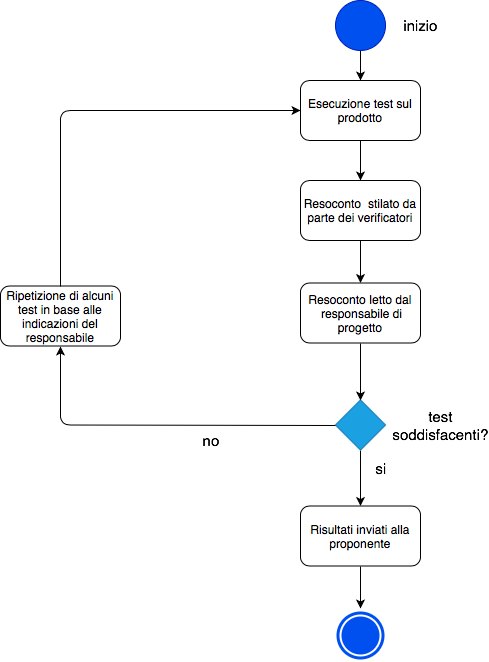
\includegraphics[scale=0.5]{Validazione.png}
	\caption{Processo di validazione}
\end{figure}
 
		
	
	